\documentclass[11pt, oneside]{book}

%%%%%%%%%%%%%%Include Packages%%%%%%%%%%%%%%%%%%%%%%%%%%
\usepackage{xcolor}
\usepackage{mathtools}
\usepackage[a4paper, total={6in, 8in}, margin=1.25in]{geometry}
\usepackage{amsmath}
\usepackage{amssymb}
\usepackage{paralist}
\usepackage{rsfso}
\usepackage{amsthm}
\usepackage{wasysym}
\usepackage[inline]{enumitem}   
\usepackage{hyperref}
\usepackage{tocloft}
\usepackage{titlesec}
\usepackage{colortbl}
\usepackage{slashed}
\usepackage{sidenotes}
%%%%%%%%%%%%%%%%%%%%%%%%%%%%%%%%%%%%%%%%%%%%%%%%%%%%%%%%


\definecolor{shadecolor}{rgb}{1,1,1}

%%%%%%%%%%%%%%%Chapter Setting%%%%%%%%%%%%%%%%%%%%%%%%%%
\definecolor{gray75}{gray}{0.75}
\newcommand{\hsp}{\hspace{20pt}}
\titleformat{\chapter}[hang]{\Huge\bfseries}{\thechapter\hsp\textcolor{gray75}{$\mid$}\hsp}{0pt}{\Huge\bfseries}
%%%%%%%%%%%%%%%%%%%%%%%%%%%%%%%%%%%%%%%%%%%%%%%%%%%%%%%%

%%%%%%%%%%%%%%%%%Theorem environments%%%%%%%%%%%%%%%%%%%
\newtheoremstyle{break}
  {\topsep}{\topsep}%
  {\itshape}{}%
  {\bfseries}{}%
  {\newline}{}%
\theoremstyle{break}
\theoremstyle{break}
\newtheorem{axiom}{Axiom}
\newtheorem{thm}{Theorem}[section]
\renewcommand{\thethm}{\arabic{section}.\arabic{thm}}
\newtheorem{lem}{Lemma}[thm]
\newtheorem{cor}{Corollary}[thm]
\newtheorem{defn}{Definition}[thm]
\newenvironment{indEnv}[1][Proof]
  {\proof[#1]\leftskip=1cm\rightskip=1cm}
  {\endproof}
%%%%%%%%%%%%%%%%%%%%%%%%%%%%%%%%%%%%%%%%%%%%%%%%%%%%%%


%%%%%%%%%%%%%%%%%%%%%%%Integral%%%%%%%%%%%%%%%%%%%%%%%
\def\upint{\mathchoice%
    {\mkern13mu\overline{\vphantom{\intop}\mkern7mu}\mkern-20mu}%
    {\mkern7mu\overline{\vphantom{\intop}\mkern7mu}\mkern-14mu}%
    {\mkern7mu\overline{\vphantom{\intop}\mkern7mu}\mkern-14mu}%
    {\mkern7mu\overline{\vphantom{\intop}\mkern7mu}\mkern-14mu}%
  \int}
\def\lowint{\mkern3mu\underline{\vphantom{\intop}\mkern7mu}\mkern-10mu\int}
%%%%%%%%%%%%%%%%%%%%%%%%%%%%%%%%%%%%%%%%%%%%%%%%%%%%%%



\newcommand{\R}{\mathbb{R}}
\newcommand{\N}{\mathbb{N}}
\newcommand{\Z}{\mathbb{Z}}
\newcommand{\Q}{\mathbb{Q}}
\newcommand{\C}{\mathbb{C}}
\newcommand{\Lg}{\mathcal{L}}
\newcommand{\Hm}{\mathcal{Hm}}
\newcommand{\Power}{\mathcal{P}}
\newcommand{\ee}[1]{\cdot 10^{#1}}
\newcommand{\spa}{\text{span}}
\newcommand{\sgn}{\text{sgn}}
\newcommand{\degr}{\text{deg}}
\newcommand{\B}{\text{B}}
\newcommand{\pd}{\partial}
\newcommand{\that}[1]{\widetilde{#1}}
\newcommand{\lr}[1]{\left(#1\right)}
\newcommand{\vmat}[1]{\begin{vmatrix} #1 \end{vmatrix}}
\newcommand{\bmat}[1]{\begin{bmatrix} #1 \end{bmatrix}}
\newcommand{\pmat}[1]{\begin{pmatrix} #1 \end{pmatrix}}
\newcommand{\rref}{\xrightarrow{\text{row\ reduce}}}
\newcommand{\txtarrow}[1]{\xrightarrow{\text{#1}}}
\newcommand{\txt}{Wald's \textit{General Relativity}}

\newcommand{\note}{\color{red}Note: \color{black}}
\newcommand{\remark}{\color{blue}Remark: \color{black}}
\newcommand{\example}{\color{green}Example: \color{black}}
\newcommand{\exercise}{\color{green}Exercise: \color{black}}

%%%%%%%%%%%%%table of contents%%%%%%%%%%%%%%%%%%%%%%%%%%%%
%\setlength{\cftchapindent}{0em}
%\cftsetindents{section}{2em}{3em}
%
%\renewcommand\cfttoctitlefont{\hfill\huge\bfseries}
%\renewcommand\cftaftertoctitle{\hfill\mbox{}}
%
%\setcounter{tocdepth}{2}
%%%%%%%%%%%%%%%%%%%%%%%%%%%%%%%%%%%%%%%%%%%%%%%%%%%%%%%%%%


%%%%%%%%%%%%%%%%%%%%%Footnotes%%%%%%%%%%%%%%%%%%%%%%%%%%%
\newcommand\blfootnote[1]{%
  \begingroup
  \renewcommand\thefootnote{}\footnote{#1}%
  \addtocounter{footnote}{-1}%
  \endgroup
}
%%%%%%%%%%%%%%%%%%%%%%%%%%%%%%%%%%%%%%%%%%%%%%%%%%%%%%%%%

%%%%%%%%%%%%%%%%%%%%%Section%%%%%%%%%%%%%%%%%%%%%%%%%%%%%
\makeatletter
\def\@seccntformat#1{%
  \expandafter\ifx\csname c@#1\endcsname\c@section\else
  \csname the#1\endcsname\quad
  \fi}
\makeatother
%%%%%%%%%%%%%%%%%%%%%%%%%%%%%%%%%%%%%%%%%%%%%%%%%%%%%%%%%

\begin{document}

	\begin{titlepage}
		\begin{center}
			\vspace*{0.5cm}
			\LARGE \color{black}
				\textbf{Majorana Zero Modes \\in Topological Superconductors}\\
			\vspace{0.5cm}			
			\Large \color{black}
			\vspace{1.5cm}

			
			
			
			\vspace{2cm}
			\LARGE
				\textbf{Jinyan Miao}\\
				\text{Department of Physics, UCLA}\\
				\hfill\break
				\LARGE Spring 2025\\
			\vspace{1cm}

		\vspace*{\fill}
		\end{center}		

	\begin{marginfigure}[-3.1cm]
		\hspace*{-2.9cm}
		
\includegraphics[scale=0.8]{hmm.pdf}
	\end{marginfigure}

	\end{titlepage}


\newpage
\tableofcontents 



\chapter{Introduction}
This note introduces Majorana fermions and how they appear in certain condensed matter theory for superconductors, and can be used for quantum computing. The idea of a fermion being its own antiparticle was first proposed by Ettore Majorana in 1937, as a special kind of solution to the Dirac equation. In particle physics, such particles must be neutral. While no fundamental Majorana fermions have been confirmed, they have been regarded as quasiparticles in solid-state systems.\\

We begin in chapter 2 with a review of the Dirac equation and how the Majorana condition arises. We show how real solutions can be obtained using the Majorana representation of gamma matrices, and how these describe neutral fermions. This sets the stage for understanding how similar structures appear in superconductors.\\

In chapter 3, we turn to the Bogoliubov–de Gennes (BdG) formalism, which describes superconductors at the mean-field level. Here, quasiparticles are superpositions of electrons and holes, and the BdG Hamiltonian leads naturally to operators that satisfy $\gamma = \gamma^\dagger$. These are Majorana zero modes (MZMs). We study the Kitaev chain, a simple 1D model that supports MZMs at its ends in the topological phase, and the Fu–Kane model, where a vortex in a 2D superconductor traps a MZM.\\

In chapter 4, we examine what happens when vortices, and the MZMs they bind, are moved around each other. This leads to non-Abelian exchange statistics of the MZMs, and the construction of the corresponding braid group, which attract a lot of interests in recent years for its potential application in topological quantum computing.\\

This note follows the structure and ideas in the review article by Steven R. Elliott and Marcel Franz \cite{Review}, but presents the material with more detailed derivations. The goal is to provide a clear and accessible entry point for students interested in the theory behind Majorana modes in condensed matter physics.

\chapter{Majorana Fermion}
\section{Dirac Equation}
To discuss Majorana fermions, we start with the Dirac equation from the particle physics point of view. Dirac equation describes dynamics of spin-half fermions,
\begin{align}
i\dot{\psi} = H_{\text{Dirac}}\psi = \left(\vec{\alpha}\cdot \vec{p}+ \beta m \right)\psi\,,
\end{align}
where $\vec{\alpha}$ is a vector of $4\times 4$ matrix, 
\begin{align}
\vec{\alpha} = (\alpha^1, \, \alpha^2,\,\alpha^3)\,,
\end{align}
and $\beta$ is another $4\times 4$ matrix. They are defined to satisfy the Clifford algebra
\begin{align}
\{\alpha^i,\, \alpha^j\} = 2\delta^{ij}\mathbb{I},\,\qquad
\{\alpha^i,\, \beta\} = 0\,,\qquad
\beta^2 = \mathbb{I}\,,
\end{align}
with $\mathbb{I}$ being the $4\times 4$ identity matrix. These are defined to ensure Lorentz invariance and that the energy spectrum reproduces the 
\begin{align}
E^2 = p^2 + m^2
\end{align}
relation. We then can define the gamma matrices
\begin{align}
\gamma^\mu = \left(\beta,\, \beta \alpha^i\right)
\end{align}
such that the Dirac equation (2.1) becomes
\begin{align}
(i\gamma^\mu \pd_\mu - m) \psi = (\gamma^\mu p_\mu -m) \psi 
= 0\,.
\end{align}
In this case, the Clifford algebra can be summarized to
\begin{align}
\{ \gamma^\mu, \, \gamma^\nu\} = 2\eta^{\mu\nu}\mathbb{I}\,,\qquad
(\gamma^\mu)^\dagger  = \gamma^0 \gamma^\mu \gamma^0
,
\end{align}
where we have added the second condition for Hermicity of the Dirac Hamiltonian. 
The matrices are not unique, but in the Dirac basis, they are 
\begin{align}
\gamma^0 = \bmat{\mathbb{I}_2 & 0 \\ 0 & -\mathbb{I}_2}\,,\qquad
\gamma^i = \bmat{0 & \sigma^i \\ -\sigma^i & 0}\,,
\end{align}
where $\mathbb{I}_2$ is the $2\times 2$ identity matrix and $\sigma^i$ are the Pauli matrices. For another example, in the Weyl basis,
\begin{align}
\gamma^\mu = \bmat{0 & \sigma^\mu \\ \bar{\sigma}^\mu & 0}\,,
\end{align}
where $\sigma^0 = \mathbb{I}_2$ and $\bar{\sigma}^\mu = (\sigma_0, -\sigma^i)$. These different representation are used to conveniently solve different physical problems. We notice that the Dirac equation (2.6) is a system of four coupled equations for a four-component bispinor $\psi$. Ettore Majorana's insight is that we can choose a basis such that the Dirac equation becomes real (with real solution) and the system of four coupled equations reduces to two independent systems of two coupled equations. Choosing such a basis does not effect the spin of the spinor, that is, we will use the Majorana basis to describe a spin-half particle-antiparticle pair, in the next section.\\

\section{Majorana Condition}
\subsection{Majorana Representation for the gamma Matrices}
As introduced in the last section, we have the gamma matrices that define the Clifford algebra, and they are used in the Dirac equation to describe the dynamics of a spin-half fermion. We consider the following basis (also called representation) of the gamma matrices:
\begin{align}
{\gamma}^0 = i \bmat{0 & -\sigma^1\\ \sigma^1 & 0}\,,\quad
{\gamma}^1 = i \bmat{0 & \sigma^0\\ \sigma^0 & 0}\,,\quad
{\gamma}^2 = i\bmat{\sigma^0 & 0 \\ 0 & -\sigma^0 }\,,\quad
{\gamma}^3 = \bmat{0& \sigma^2 \\ -\sigma^2&0 }\,.
\end{align}
This representation is called the Majorana representation. 
%\footnote{If not specified otherwise, we use the notation $\gamma^\mu$ for gamma matrices in the Majorana representation for the rest of this text.} 
It is trivial to show that these matrices satisfy (2.7). While they also satisfy
\begin{align}
(\gamma^\mu)^* = -\gamma^\mu\,,
\end{align}
as they are all imaginary. In fact, there are other choices of gamma matrices that satisfy the Clifford algebra and (2.11), and they are all equivalent Majorana representation. Under condition (2.11), we know that $i\gamma^\mu$ is real, and thus 
\begin{align}
(i\gamma^\mu \pd_\mu - m) \psi = 0
\end{align}
is a completely real coupled PDE system. Thus it admits real solution $\psi$ which satisfies 
\begin{align}
\psi^* = \psi\,.
\end{align}
Eq.\,(2.12) is one way of writing the Majorana equation with a real operator $(i\gamma^\mu \pd_\mu - m)$, and its solution $\psi$ represents a Majorana fermion. We emphasize that the Majorana representation of the gamma matrices is not unique.\\
%Now we investigate how the system is decoupled. Combining (2.10) with (2.12), 
%\begin{align}
%\left(
%\bmat{\sigma^0\pd_2 & \pd_1 \sigma^0 + \pd_0 \sigma^1 + \pd_3 \sigma^2\\
%\pd_1 \sigma^0 - \pd_0 \sigma^1- \pd_3 \sigma^2 &-\sigma^0 \pd_2}-m\mathbb{I}
%\right)\bmat{\xi_1\\ \xi_2} = 0\,,
%\end{align}
%where $\xi_1$ and $\xi_2$ are $2$-component vectors. \\
%Now we define, up to some normalization of the states,
%\begin{align}
%\eta_1 = \xi_1 + \xi_2 \,,\qquad
%\eta_2 = \xi_1 - \xi_2\,.
%\end{align}



\subsection{Gauge and Charge Conjugation Symmetries}
Now we go back a little and discuss one of the key properties of the Dirac field. The Lagrangian (density) whose equation of motion has the form of (2.1) is 
\begin{align}
\mathcal{L} = \bar{\psi}(i \gamma^\mu \pd_\mu - m) \psi\,,
\end{align}
where 
\begin{align}
\bar{\psi}\coloneqq \psi^\dagger \gamma^0
\end{align}
is the Dirac adjoint of the field $\psi$. It is easy to verify that the equation of motion 
\begin{align}
\frac{\pd \mathcal{L}}{\pd \bar{\psi}} - \frac{\pd}{\pd x^\mu}\frac{\pd \mathcal{L}}{\pd (\pd_\mu \bar{\psi})} = 0
\end{align}
leads to the Dirac equation (2.1). From the Lagrangian we see that the field has a global $U(1)$ symmetry 
\begin{align}
\psi(x) \to e^{i\theta}\psi(x) \,,\qquad
\bar{\psi}(x) \to e^{-i\theta}\bar{\psi}(x) \,,
\end{align}
for some constant $\theta \in \R$. Localising this symmetry implies promoting the constant $\theta$ to be a general function $\theta(x)$ in spacetime. In this case, to attain the local $U(1)$ symmetry,
\begin{align}
\psi(x) \to e^{i\theta(x)}\psi(x) \,,\qquad
\bar{\psi}(x) \to e^{-i\theta(x)}\bar{\psi}(x) \,,
\end{align}
it is required to replace the covariant derivative by
\begin{align}
\pd_\mu \to D_\mu\coloneqq \pd_\mu - iqA_\mu(x)
\end{align}
where we identify $q$ as the charge of the fermion, and $A_\mu(x)$ is a gauge field. The standard interpretation is that this couples the Dirac fermion to the electromagnetic field and thus describes charged particles. After the replacement of the covariant derivative, the Dirac equation has the form
\begin{align}
(i\slashed{\pd} - q\slashed{A} - m) \psi= 0
\end{align}
with $\slashed{T} = T_\mu \gamma^\mu$. Eq. (2.20) allows us to discuss charge conjugation symmetry of the Dirac field - One wishes to find a charge-conjugation solution to (2.20), which is a solution that describes the field $\psi$ but with an opposite charge. That is, we seek solution of the form
\begin{align}
(i\slashed{\pd} + q\slashed{A} - m) \psi^c= 0\,.
\end{align}
Complex conjugating (2.20) one finds
\begin{align}
\left(-i(\gamma^\mu)^*\pd_\mu - q(\gamma^\mu)^*A_\mu - m\right)\psi^* = 0\,.
\end{align}
Now we see that if we can find a $4\times 4$ matrix $C$ that satisfies
\begin{align}
C^{\dagger} \gamma^\mu C = -(\gamma^\mu)^*
\end{align}
and define
\begin{align}
\psi^c = C \psi^*\,,
\end{align}
then charge conjugating (2.22) gives (2.21). We note that the charge conjugation operator $C$ and the field $\psi^c$ are still well defined when the coupling, or charge, $q$ is set to zero.\\

We discussed in section 2.2.1 that the Dirac equation has completely real solution under Majorana representation of the gamma matrices. We have also discussed that there are other representations of the gamma matrices with other solutions to the Dirac equation. In general, any two representations of gamma matrices are related by a similarity transformation defined by a unitary matrix $U$, 
\begin{align}
\gamma^\mu = U \that{\gamma}{}^\mu U^\dagger\,,
\end{align}
then if $\that{\psi}$ is a solution (under the $\that{\gamma}{}^\mu$ basis), 
\begin{align}
\psi = U \that{\psi}
\end{align}
is also a solution. If the tilde representation is the Majorana representation, and we choose to work in the non-tilde representation, then we will need to rewrite the Majorana condition (2.13) in the non-tilde representation to check whether our solution to the Dirac equation represents a Majorana fermion. We will see in the following that this can be related to the charge conjugation operator defined by (2.23). Consider we have $\that{\psi}$ satisfying the Majorana condition (2.13) (so $\that{\gamma}^\mu$ satisfies (2.11)), then combining (2.13) and (2.26), we find that, if $\psi$ is a solution (under the non-tilde representation) that satisfies Majorana condition,
\begin{align}
U^\dagger \psi = \that{\psi} = \that{\psi}^* = (U^\dagger \psi)^*\,,
\end{align}
that is 
\begin{align}
\psi = UU^T \psi^*\,.
\end{align}
Here $UU^T$ is unitary as $U$ is unitary. Thus we can use a unitary matrix $C$ defined by 
\begin{align}
C \coloneqq UU^T
\end{align}
such that 
\begin{align}
\psi = C \psi^*
\end{align}
is the Majorana condition for $\psi$. Now we show that the unitary matrix $C$ is the one characterized by (2.23). Using (2.29), (2.25), and (2.11), we find
\begin{align}
C^{\dagger}\gamma_\mu C = U^* U^\dagger  \gamma_\mu  UU^T =  U^* \that{\gamma}_\mu U^T =-U^* \that{\gamma}_\mu^* U^T = -(\gamma^\mu)^*  \,,
\end{align}
which is exactly (2.23). Now using (2.24) and (2.30),
\begin{align}
\psi^c = C{\psi}^* = \psi\,.
\end{align}
This is the Majorana condition for $\psi$ in arbitrary basis, and it defines a Majorana fermion: A fermion that is its own antiparticle. We notice that in the Majorana basis, the charge conjugation operator is the identity. Furthermore, since we now that $\psi = \psi^c$ for a Majorana fermion, it is necessary that it carries zero charge as we shall have $q= -q$.\\

A key note here is that the Majorana condition (2.32) involves the time-dependent solution $\psi$ to the Dirac equation. For a energy eigenstate $\phi_E$ that solves the stationary Dirac equation
\begin{align}
E\phi_E = (\vec{\alpha}\cdot \vec{p} + \beta m ) \phi_E\,,
\end{align}
we know that $\psi = e^{-iEt}\phi_E$ is the corresponding time-dependent fermionic wavefunction, and it is not necessary to satisfy the Majorana condition. The charge conjugated wavefunction has the form
\begin{align}
(e^{-iEt}\phi_E)^c = C(e^{-iEt}\phi_E)^*=e^{iEt}C\phi_E^* \,,
\end{align}
thus we say
\begin{align}
C\phi_{E}^* = \phi_{-E}\,.
\end{align}
We therefore see that (2.32) can be satisfied with an energy eigenstate $\phi_0$ that has energy $E=0$. This leads to the concept of Majorana zero modes which we will discuss in details in chapter 3. 

%For a real solution, we see that
%\begin{align}
%\psi^c = C \bar{\psi}^T =-\gamma^0 C \psi^*= -\gamma^0 C \psi\,.
%\end{align}

\subsection{Decoupling of Dirac Equation}
Here we will show that Majorana condition (2.32) decouples the system of four equations into two independent systems of two coupled equations. The solution $\psi$ of the Dirac equation is a four-component bispinor. In the Weyl representation (2.9) of the gamma matrices, we can write
\begin{align}
\psi = \bmat{\psi_{\text{L}} \\ \psi_{\text{R}}}
\end{align}
where the spin of the spinor $\psi_{\text{R}}$ aligns with its momentum, and that of $\psi_{\text{L}}$ anti-aligns with its momentum. $\psi_{\text{L/R}}$ are the left- and right-handed projections of $\psi$. Then we can write the four coupled equations as
\begin{align}
\begin{cases}
(i\pd_t - \vec{p}\cdot \vec{\sigma})\psi_{\text{R}} - m\psi_{\text{L}} = 0\\
(i\pd_t + \vec{p}\cdot \vec{\sigma})\psi_{\text{L}} - m\psi_{\text{R}} = 0\\
\end{cases}\,.
\end{align}
One can verify that the charge conjugation operator in this basis has the form
\begin{align}
C = \bmat{0 & i\sigma^2 \\ -i\sigma^2 & 0}\,.
\end{align}
Thus we can compute
\begin{align}
\psi^c = C\psi^* = 
 \bmat{0 & i\sigma^2 \\ -i\sigma^2 & 0} 
\bmat{\psi_{\text{L}}^*\\ \psi_{\text{R}}^*} = i\sigma^2\bmat{\psi_{\text{R}}^*\\ -\psi_{\text{L}}^*}\,.
\end{align}
Thus if we have (2.32) satisfied, (2.37) becomes 
\begin{align}
\begin{cases}
(i\pd_t - \vec{p}\cdot \vec{\sigma}) \psi_{\text{R}} - im_{\text{R}} \sigma^2 \psi_{\text{R}}^*=0\\
(i\pd_t + \vec{p}\cdot \vec{\sigma}) \psi_{\text{L}} - im_{\text{L}} \sigma^2 \psi_{\text{L}}^*=0
\end{cases}\,,
\end{align}
where we have indicated by subscripts that the mass for $\psi_{\text{R}}$ is not required to be equal to that of $\psi_{\text{L}}$ for Majorana fermions. Thus we see that the dynamics of and left- and right-handed spinors are independent. The Majorana fields can now be expressed as
\begin{align}
\psi_1 = \bmat{
\psi_{\text{L}}\\
-i \sigma^2 \psi_{\text{L}}^*
}\,,\qquad
\psi_2 = \bmat{
i \sigma^2 \psi_{\text{R}}^*\\
\psi_{\text{R}}
}\,.
\end{align}


\subsection{Field Theory Description}
In the formalism of the second quantization scheme, solutions to the Dirac equation are field operators, which we denote as $\hat{\psi}$. Quantizing the free theory, the field operator has the form
\begin{align}
\hat{\psi}(x) = \sum_{E>0}a(E)\,e^{-iEt}\phi_E(\vec{x}) + \sum_{E<0}b^\dagger(-E)\,e^{-iEt}\phi_E(\vec{x})\,,
\end{align}
where $\phi_E(\vec{x})$ is an eigenstate of the stationary Dirac equation at energy $E$, and $a^\dagger(E)$ and $b^\dagger(E)$ are creation operators for particle and antiparticle with energy $E$, respectively. The creation and annihilation operators for particles and antiparticles satisfy the usual canonical anticommutation relations,
\begin{align}
\{a_r(E),\, a_s^\dagger(E')\} = \delta_{r,s}\, \delta_{E,E'}\,,\qquad
\{b_r(E),\, b_s^\dagger(E')\} = \delta_{r,s}\, \delta_{E,E'}\,\qquad
\end{align}
(with all other anticommutators vanish, here $r$ and $s$ subscripts denote the spin). These translate to the equal-time anticommutation relations for the field operator, 
\begin{align}
\{\hat{\psi}_a(x),\, \hat{\psi}_b^\dagger(x')\}|_{x^0=x'{}^0} = \delta_{ab}\, \delta(\vec{x}-\vec{x}')\,,\qquad
\{\hat{\psi}_a(x),\, \hat{\psi}_b(x')\}|_{x^0=x'{}^0} = 0\,,
\end{align}
with $a,b$ labeling the spinor components. To construct the Majorana fermion field, we have learned that Majorana fermion is its own antiparticle, thus we demand $a_E = b_E$, which leads to 
\begin{align}
&\hat{\psi}(x) = \sum_{E>0}a(E)\,e^{-iEt}\phi_E(\vec{x}) + \sum_{E<0}a^\dagger(-E)\,e^{-iEt}\phi_E(\vec{x})\,.                                                                                                                                                                                                                                                                                                                                                                                                                                                                                                                                                                                                                                                                                                                                                      
\end{align}
Then in the Majorana basis, $C = \mathbb{I}$, combining that with (2.35) we find 
\begin{align}
\hat{\psi}^\dagger(x) 
&= \sum_{E>0}\, a^\dagger(E)\, e^{iEt}\, \phi_{-E}(\vec{x}) +\sum_{E<0}a(-E)\, e^{iEt}\, \phi_{-E}(\vec{x}) = \hat{\psi}(x)
\end{align}
and 
\begin{align}
\{\hat{\psi}_a(x),\, \hat{\psi}_b(x')\}|_{x^0=x'{}^0} = \delta_{ab}\, \delta(\vec{x}-\vec{x}')
\end{align}
for a Majorana fermionic field.

%\subsection{Fourier Expansion}
%We now use $\that{\psi}$ to denote a Dirac field that satisfies the Majorana condition (2.13), that is $\that{\psi}$ is real.  

\section{Majorana Basis in Solid-state Physics}
We have seen from the point of view of particle physics that Majorana fermions correspond to the real solutions to the Dirac equation, or, correspond to the class of solutions with the property that particle being its own antiparticle. From the solid-state physics point of view, perhaps the only fermionic particles that are of interest are the electrons. Majorana fermions, on the other hand, can occur as emergent quasiparticles to describe excitations in many-body quantum system, as we will see in the next chapter.\\

Before we move on to the examples, we first discuss how Majorana fermions are described from the point of view of solid-state physics. We have learned from the particle physics point of view that Majorana fermion is its own particle, thus we expect to see that the relation $\gamma^\dagger = \gamma$ for the creation and annihilation operators for such a particle. For electrons, on the other hand, they are defined by the usual fermionic creation and annihilation operators $c_j^\dagger$ and $c_j$ that satisfy the anticommutation relations
\begin{align}
\{c_i^\dagger,\, c_j^\dagger\} = \{c_j,\, c_j\} = 0\,,\qquad
\{c_i^\dagger,\, c_j\} = \delta_{ij}\,,
\end{align}
where the subscripts $i,j$ encode information about position degree of freedom and quantum numbers of the electron. In the formalism of second quantization scheme, the Hamiltonian describing systems consisting of electrons is formed by kinetic terms that are bilinear in $c$'s, and interaction terms that are higher order in $c$'s. The operators $c$ and $c^\dagger$ are in general complex, and we are free to perform a change of basis, 
\begin{align}
c_j = \frac{1}{2}\left( \gamma_{j1}+i \gamma_{j2}\right) \,,\qquad
c^\dagger_j  = \frac{1}{2}\left( \gamma_{j1}-i\gamma_{j2}\right)\,.
\end{align}
Inverting these relations, we find
\begin{align}
\gamma_{j1} = c_j + c_j^\dagger \,,\qquad
\gamma_{j2} = i\left(c_j^\dagger-c_j\right)\,.
\end{align}
Straight from the definition, we see that the operators $\gamma_{j\alpha}$ satisfy 
\begin{align}
\gamma^\dagger_{i\alpha} = \gamma_{i\alpha}\,,
\end{align}
and thus they are the creation and annihilation operators for Majorana fermion. From the electron anticommutation relations, the $\gamma_{i\alpha}$ operators further satisfy
\begin{align}
\{\gamma_{i\alpha},\, \gamma_{j\beta}\} = 2\delta_{ij}\delta_{\alpha\beta}\,.
\end{align}
From the change of basis structure that defines the $\gamma_{i\alpha}$ operators, we can loosely interpret the $\gamma_{i\alpha}$ as the real and imaginary parts of the $c_j$ operators. Thus we interpret this structure as follows, an electron in space consists of two Majorana fermions intertwined in space. Therefore, in the case where the two Majorana fermions comprising an electron cannot be spatially separated and detected individually, such a transformation merely complicate things. However, we shall see in the next chapter that the Majorana basis defined by the $\gamma_{i\alpha}$ operators is useful in analyzing topological superconductors, where we have spatially isolated Majorana fermions and we can discuss the exchange statistics of them. 


\chapter[Introduction to Topological Superconductivity]{Introduction to Topological\\ Superconductivity}
We have discussed the definition and some property of the Majorana fermion, now we shall discuss how Majorana fermions can be used naturally in theories for superconductors. Just as how  electron-hole pairs are used in Fermi liquid theory, Majorana fermions can occur in certain theory as emergent quasiparticles, and they describe the collective excitations of the quantum many-body state in interacting electronic systems.

\section{The BdG Theory}
We start by reviewing the Bogoliubov-de Gennes (BdG) formalism. The BdG formalism is used to describe solids with superconducting order, and we will see how majorana fermions can arise in superconductors under this theory. \\

\subsection{The BdG Hamiltonian}
Superconductivity arises when electrons in metal experience attractive interaction. The minimal model that describe such a superconductor is characterized by the Hamiltonian in $d$-dimension,
\begin{align}
H = \int d^d r\left( h_0^{\sigma \sigma'}(\vec{r})\, c_{\sigma \vec{r}}^\dagger c_{\sigma'\vec{r}} - V n_{\uparrow \vec{r}}n_{\downarrow \vec{r}}\right)\,.
\end{align}
Here $c_{\sigma \vec{r}}^\dagger$ creates an electron with spin $\sigma$ at the spatial point $\vec{r}$, and $n_{\sigma \vec{r}}\coloneqq c_{\sigma \vec{r}}^\dagger c_{\sigma \vec{r}}$ is the number operator. $V$ is taken to be strictly positive such that it represents attractive interaction between electrons. In the simplest case of free electrons, 
\begin{align}
h_0^{\sigma \sigma'} (\vec{r}) = \left( 
-\frac{\hbar^2 \nabla^2}{2m_{\text{eff}}} -\mu
\right)\, \delta_{\sigma \sigma'}\,,
\end{align}
where $m_{\text{eff}}$ represents the electron band mass and $\mu$ is the chemical potential. Thus the first term in the Hamiltonian describes the kinetic energy of the electrons and single-electron potential. The second term in the Hamiltonian describes the interaction. We see that (3.1) involves quartic term $n^2$, thus we take the Bogoliubov mean-field decoupling approximation by assuming the dominant physics is pairing, 
\begin{align}
-n_\uparrow n_\downarrow = c^\dagger_\uparrow c^\dagger_\downarrow
c_\uparrow c_\downarrow \approx 
\langle c_{\uparrow}^\dagger c_\downarrow^\dagger\rangle c_\uparrow c_\downarrow + c_\uparrow^\dagger c_\downarrow^\dagger \langle c_\uparrow c_\downarrow\rangle - \langle c_\uparrow^\dagger c_\downarrow^\dagger\rangle \langle c_\uparrow c_\downarrow\rangle\,.
\end{align}
The expectation values are taken with respect to the BdG mean-field Hamiltonian,
\begin{align}
H_{\text{BdG}} = \int d^d r\left( h_0^{\sigma \sigma'}(\vec{r})\, c_{\sigma r}^\dagger c_{\sigma'\vec{r}}
+\left(
\Delta(\vec{r})\, c_{\uparrow\vec{r}}^\dagger c_{\downarrow\vec{r}} + \text{H.\,c.}
\right)-\frac{1}{V}|\Delta(\vec{r})|^2
\right)\,.
\end{align}
which follows from (3.1) if we define
\begin{align}
\Delta(\vec{r}) \coloneqq V\langle c_{\uparrow\vec{r}}c_{\downarrow \vec{r}}\rangle\,.
\end{align}
To see how this is connected to the Majorana fermion, we write the Hamiltonian in the form
\begin{align}
H_{\text{BdG}} = \int d^d r\left({\psi}_{\vec{r}}^\dagger\, \mathcal{H}_{\text{BdG}}\,(\vec{r}){\psi}_{\vec{r}} - \frac{1}{V}|\Delta (\vec{r})|^2\right)
\end{align}
where ${\psi}_{\vec{r}}$ is a four-component Nambu spinor,
\begin{align}
{\psi}_{\vec{r}} \coloneqq \bmat{c_{\uparrow\vec{r}} \\
c_{\downarrow\vec{r}}\\
c_{\downarrow\vec{r}}^\dagger\\
-c_{\uparrow\vec{r}}^\dagger} = \bmat{\that{\psi}_{\vec{r}} \\ i\sigma^y \that{\psi}_{\vec{r}}^*}\,,
\end{align}
and $\mathcal{H}_{BdG}$ is the BdG Hamiltonian 
\begin{align}
\mathcal{H}_{\text{BdG}}(\vec{r}) = \bmat{h_0(\vec{r}) & \Delta(\vec{r}) \\ \Delta^*(\vec{r}) & -\sigma^y \,h_0^*(\vec{r})\, \sigma^y}\,,
\end{align}
Now we see that the Nambu spinor has a structure that we have seen in (2.38). That is, the Nambu spinor satisfies the Majorana condition (2.32), given that the charge conjugation matrix is defined by 
\begin{align}
C = \tau^y  \sigma^y\,.
\end{align}
where $\vec{\tau} = (\tau^x, \, \tau^y,\, \tau^z)$ is again the vector of Pauli matrices, but they act on the Nambu space, which has a two-component structure defined by the second equality of ${\psi}_{\vec{r}}$. We note that the Majorana property arises from the fact that the lower two components of the Nambu spinor are related to the upper two, as indicated in (3.7), and this structure follows from the form of the mean-field Hamiltonian in (3.4). Thus in the BdG formalism, it is required to employ Majorana fermions to describe the excitations of quasiparticle in the superconductor. This is in contrast with what we have discussed in chapter 2 where Majorana fermion is merely one of the solutions to the Dirac equation. \\

\subsection{Majorana Zero Mode in Superconductors}
Now we have seen that the description of quasiparticle excitations in the BdG theory for superconductors possess all key features of Majorana fermions. This involves the discussion of the Nambu spinor $\psi_{\vec{r}}$ that we defined in (3.7). We have also learned at the end of section 2.2.2 that the zero energy eigenstate $\phi_0$ of the Hamiltonian $\mathcal{H}_{\text{BdG}}$ should also give us some interesting result as it also satisfies the Majorana condition. We will devote the next few sections to discuss the properties of the zero energy modes, called the Majorana zero modes. \\


First we would like to study the energy eigenstates of the Hamiltonian defined in (3.8). That is, consider here eigenfunction $\phi_n(\vec{r}) = (u_{n\uparrow}(\vec{r}),\, u_{n\downarrow}(\vec{r}) ,\, v_{n\uparrow}(\vec{r}),\, v_{n\downarrow}(\vec{r}))$ with eigenvalue $E_n$ that satisfies
\begin{align}
\mathcal{H}_{\text{BdG}}(\vec{r})\, \phi_n(\vec{r}) = E_n \phi_n(\vec{r})\,.
\end{align}
Then we define a creation operator $a_n^\dagger$, which creates a Bogoliubov quasiparticle with energy $E_n$,
\begin{align}
a^\dagger_n = \int d^d r \, \phi_n^\dagger(\vec{r})\, \psi_{\vec{r}}\,,
\end{align}
such that we can rewrite $H_{\text{BdG}}$ in terms of energy levels, 
\begin{align}
H_{\text{BdG}} = \sum_{E_n\geq 0} E_n a_n^\dagger a_n + E_g\,,
\end{align}
where $E_g$ is a constant for ground state energy. Now we focus on the zero energy mode for $\mathcal{H}_{\text{BdG}}$, which is characterized by
\begin{align}
\mathcal{H}_{\text{BdG}}(\vec{r})\, \phi_0(\vec{r}) = 0\,.
\end{align}
We have seen that the Nambu spinor $\psi_{\vec{r}}$ are Majorana fermions, then for the zero energy mode, combining the Majorana condition, (2.34), and (2.35), we find
\begin{align}
\bmat{u_{0\uparrow}(\vec{r})\\ 
u_{0\downarrow}(\vec{r}) \\ 
v_{0\uparrow}(\vec{r})   \\
v_{0\downarrow}(\vec{r})} = \phi_0(\vec{r}) = C\phi_0^*(\vec{r}) = 
\tau^y\sigma^y\phi_0^*(\vec{r}) =
\bmat{
-v^*_{0\downarrow}(\vec{r})  \\
v^*_{0\uparrow}(\vec{r})   \\
u_{0\downarrow}^*(\vec{r}) \\ 
-u_{0\uparrow}^*(\vec{r})
}\,.
\end{align}
Then the creation and annhilation operator for the Bogoliubov quasiparticle corresponding to this zero energy mode can be constructed using (3.11), and it is easy to check that 
\begin{align}
a_0&=\int d^d r \left(
u^*_{0\uparrow}c_{\uparrow} + 
u_{0\downarrow}^* c_{\downarrow} + 
v_{0\downarrow}^* c_{\downarrow}^* -v_{0\downarrow}^* c_{\uparrow}^*
\right)  
= \int d^d r \left(c_{\uparrow}^* u_{0\uparrow} + c_{\downarrow}^*u_{0\downarrow} + c_{\downarrow}v_{0\uparrow} - c_{\uparrow}v_{0\downarrow}\right)= a^\dagger_0\,.
\end{align}
The consequence of (3.15) is that the number operator for the zero energy mode cannot be formed in the usual way, as the value of $n_0 = a^\dagger_0 a_0 = a_0 a_0$ is fixed by the anticommutation relation $\{a_0, a_0\}$. The zero energy manifold is also degenerate, because if $|0\rangle$ is a zero energy mode, then $a^\dagger_0|0\rangle$ is another one. Thus we conclude that in the presence of MZM, the ground state of the system is degenerate. We also say that these MZMs are topologically protected by the minigap (energy gap) separating it from all other nonzero energy states. The zero mode cannot acquire a nonzero energy energy by any continuous deformation of the Hamiltonian that does not close the minigap. \\

Now we have seen how Majorana fermions naturally arise in a superconductor theory, and why the Majorana zero modes are of special interests. The next step we will take is to look at the system from another angle, using the Majorana basis that we considered in section 2.3. In the next section, we will focus on another model where we will see that the MZMs occur in pairs and can be spatially isolated, and will analyze it using the Majorana basis approach. Then we will come back in chapter 4 and revisit the BdG theory by considering the Fu-Kane model, where the BdG Hamiltonian has a given form, and we will discuss the exchange statistics and the braiding of the MZMs in that model. As a special note, the following discussion focuses on Majorana zero modes (MZMs) in topological superconductors, where these phenomena associated with MZMs in solids occur only in one- and two-dimensional systems and have no direct analog in high-energy physics.\\





%This reflects the fact that the system contains an integral number of electrons. Then we can discuss the exchange statistics of the MZMs when they are spatially separated.\\





%%%%%%%%%%%%%%%%%%%%%%%%%%%%
%%%%%%%%%%%%%%%%%%%%%%%%%%%%
%%%%%%%%%%%%%%%%%%%%%%%%%%%%
%\newpage
%Assembling one shall find 
%\begin{align}
%\that{\psi}_0^\dagger = \that{\psi}_0
%\end{align}
%and thus the zero-mode particle is its own antiparticle. \\
%
%Just to briefly go over, the Majorana zero mode has the following properties:
%\begin{enumerate}
%\item The ground state of the zero mode is degenerate because it takes zero energy to create such a state. That is, if $|0\rangle$ is a ground state then so is $\that{\psi}_0|0\rangle$. 
%\item  The discussion above makes it clear that if a
%Majorana zero mode exists in a system then it is
%topologically protected, provided that there is an
%energy gap separating it
%from all other states. The reason is that the zero
%mode cannot acquire a nonzero energy $E_0$ by any
%continuous deformation of the Hamiltonian that
%does not close the energy gap. If this were so then
%it would require another mode to appear at energy $-E_0$, in violation
%of the unitary evolution.\\
%\item A situation of interest arises when the two MZMs are spatially separated. If there are several MZMs in the system, it can be shown that their exchange statistics is complicated, and that the MZMs should be described as non-Abelian anyons, which underlines the potential significance of MZMs for topological quantum computation. 
%\end{enumerate}


\section{The Kitaev Chain Model}

The Kitaev chain model is a one-dimensional toy model, from which we can study the properties of the MZMs. It consists of spinless fermions, so it was initially considered to be unphysical, but was later found that electrons subjected to spin-orbital coupling and the Zeeman field would behave like spinless fermions. We start by considering the Hamiltonian 
\begin{align}
H = \sum_{j=1}^{N-1} 
-t \left(c_j^\dagger c_{j+1} + \text{H.c.}\right) +
\sum_{j=1}^N- \mu \left( c_j^\dagger c_j - \frac{1}{2}\right) +
\sum_{j=1}^{N-1}\Delta \left( c_j^\dagger c_{j+1}^\dagger + \text{H.c.}\right)\,,
\end{align}
for a one-dimensional chain of spinless fermions, with creation operators $c_j$ at each site, a total of $N$ sites. The first sum in the Hamiltonian represents the hopping between sites with $t$ being the hopping amplitude; the second sum controls the filling on the chain by the chemical potential $\mu$; and the third sum represents the nearest-neighbor pairing with paring amplitude $\Delta \in\R$. Open boundary condition is considered here. We perform a change of basis defined by (2.49) to rewrite the Hamiltonian
\begin{align}
H = \frac{i}{2}\sum_{j=1}^{N}  -\mu \gamma_{j2}\gamma_{j1} +\frac{i}{2} \sum_{j=1}^{N-1} \left((t+\Delta)\gamma_{j2}\gamma_{(j+1)1} + (-t+\Delta) \gamma_{(j+1)2}\gamma_{j1}\right)\,.
\end{align}
Again, the Majorana operators $\gamma$'s are creation and annihilation operators for Majorana fermions that satisfy $\gamma = \gamma^\dagger$. 
%%%%%%%%
%%%%%%%%
The goal of studying this model is to understand how Majorana fermions occur in pairs, and how MZMs can be spatially isolated. Here we analyze two important phases in this model: The trivial phase and the topological phase. \\
%%%%%%%%
%%%%%%%%


For the trivial phase, we consider $\Delta = t = 0$. In this case, we have only the terms for energies of individual sites left, that is, 
\begin{align}
H = \sum_{j=1}^N -\frac{i\mu}{2}\gamma_{j2}\gamma_{j1} = \sum_{j=1}^{N}-\mu \left( c_j^\dagger c_j - \frac{1}{2}\right)\,.
\end{align}
Depending on the sign of the chemical potential, the ground state of the system corresponds to either having all sites occupied or unoccupied. From the first equality in (3.18), we see that two Majorana operators of different kinds are coupled at the same site $j$.\\

In contrast, one of the topological phase is obtained by having $\Delta = t$ with $\mu = 0$. The Hamiltonian in this case is
\begin{align}
H = \sum_{j=1}^{N-1} it \gamma_{j2}\gamma_{(j+1)1}= \sum_{j=1}^{N-1} 2t\left( a^\dagger_{j} a_j -\frac{1}{2}\right)\,,
\end{align}
with another change of basis defined by the operators
\begin{align}
a_j = \frac{1}{2}\left(\gamma_{j2}+i\gamma_{(j+1)1}\right)\,,\qquad
a_j^\dagger = \frac{1}{2}\left( \gamma_{j2} - i\gamma_{(j+1)1}\right)\,,
\end{align}
for $j \in \N_{N-1}$. In this phase, Majorana operator at site $j$ is paired with another one of different kind at site $j+1$. Together they describe a system of $N-1$ Bogoliubov quasiparticles (created by thje $a_j^\dagger$'s). The ground state of this phase is an $a_j$ vacuum with energy $E_g = -(N-1)t$. There is one pair of Majorana fermions which does not occur in the Hamiltonian, $\gamma_{N2}$ at site $N$ and $\gamma_{11}$ at site $1$, they occur at the two ends of the chain. Since they do not appear in the Hamiltonian, they represent MZMs. The corresponding quasiparticle creation operator for this pair of MZM is
\begin{align}
a_N^{\dagger} = \left( \gamma_{N2} - i \gamma_{11}\right)\,.
\end{align}
This pair of MZMs should be viewed as a single Dirac fermion delocalized at the two ends of the system. As the presence of such a Dirac fermion does not change the total energy of the system, the ground state in this phase is two-fold degenerated. \\


\begin{figure}[h]
  \centering
  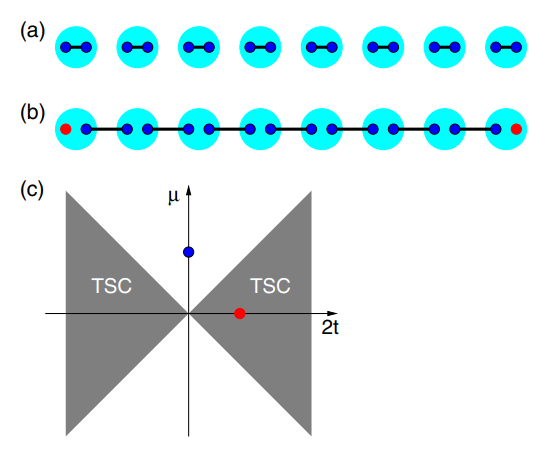
\includegraphics[scale=0.6]{1}
  \caption{\small (a) and (b) depict the trivial and topological phase in the Kitaev Chain, respectively. (c) depicts the $(2t,\mu)$-phase diagram of the Kitaev chain. The topological phase is labeled as TSC and is shaded in the diagram, where we find the red dot as the point corresponds to the topological phase discussed in the text. The blue dot corresponds to the trivial phase discussed in the text. (Figure adapted from \cite{Review})\normalsize} 
\end{figure}



The schematic diagrams of the two phases are depicted in Fig.\, 3.1(a) and (b). In the trivial phase, the two Majoranas at site $j$ bound into an ordinary fermion, while in the topological phase, two Majoranas at neighboring sites bound into an ordinary fermion, leaving the two Majoranas at the ends of the chain unpaired. To understand the reason why (3.19) describe a topological phase, we have to rewrite (3.16) in momentum space with a periodic boundary condition (identifying site $j+1$ as site $1$, so the hopping sum and paring sum in $H$ also include terms relating site $j+1$ and site $1$). First we write
\begin{align}
c_j = \frac{1}{\sqrt{N}}\sum_q e^{iqj} c_q\,,\qquad
c_j^\dagger = \frac{1}{\sqrt{N}}\sum_q e^{-iqj} c_q^\dagger\,,
\end{align}
with $q = 2\pi n/N$ for $n \in \{0,1\cdots, N-1\}$. Then we see that 
\begin{align}
\sum_{j=1}^{N}c_j^\dagger c_{j+1}c_j^\dagger c_{j+1} = 
\sum_{j=1}^{N} \sum_{q,\,q'} \frac{1}{N}e^{-iqj}e^{iq'(j+1)} c_q^\dagger c_{q'} =\frac{1}{N}\sum_{q,\,q'}e^{iq'}c_q^\dagger c_{q'} \sum_{j=1}^N e^{-ij(q-q')}\,.
\end{align}
We can use the orthogonality condition
\begin{align}
\sum_{j=1}^N e^{ij(q'-q)} = N\delta_{q,q'}\,,
\end{align}
such that 
\begin{align}
\sum_{j=1}^{N}c_j^\dagger c_{j+1}c_j^\dagger c_{j+1} = \sum_q e^{iq} c_q^\dagger c_q\,.
\end{align}
Combining with its Hermitian conjugated term, we find
\begin{align}
\sum_{j=1}^N \left(c_j^\dagger c_{j+1} + c_{j+1}^\dagger c_j\right) = \sum_q 2\cos(q) \, c_q^\dagger c_q\,.
\end{align}
Using similar treatment, we find (3.16) in momentum space under periodic boundary condition, 
\begin{align}
H =\sum_q \left(
-(2t\cos(q)+ \mu) \,c_q^\dagger c_q + \Delta (i \sin(q)\, c_q c_{-q} + \text{H.c.})
\right)\,.
\end{align}
Thus the excitation spectrum in momentum space of this system has the form
\begin{align}
E(q) = \pm \sqrt{(2t\cos(q) +\mu)^2 + (2\Delta \sin(q))^2}\,.
\end{align}
By the principle of adiabatic continuity, two systems belong to the same phase if they can be smoothly deformed into one another without closing the energy gap or breaking a symmetry. In this sense, by (3.28) we see that the system, if assumed to be in the superconducting phases ($\Delta\neq 0$), remains gapped unless $2t =\pm \mu$. Thus the $2t = \pm \mu$ curve mark the phase boundary of the system. The two phases discussed above now can be identified in the corresponding regions to the phase diagram depicted in Fig.\,3.1(c). The two phases are distinguished by the presence or absence of unpaired MZMs at the ends in the geometry with open boundary conditions. However, it is indeed possible to distinguish the topological phase from the trivial phase by studying the bulk of the system only, which involves defining a topological invariant $\mathcal{M}$ of the system, called the Majorana number. This part is beyond the scope of this note and we refer the interested reader to the Kitaev's original paper on this model \cite{KitaevChain}. \\

We have studied that the MZMs come in pairs in the Kitaev chain model. In particular, in the topological phase, the MZMs can be spatially isolated at the boundary of the one-dimensional geometry. We will see in the next chapter, where we go back to the BdG theory and study the Fu-Kain model, how one can make use of the isolated MZMs for storing and manipulating quantum information.


\chapter{Exchange Statistics of MZMs}
We were introduced to the idea of Majorana zero modes (MZMs) and studied how to find a pair of spatially isolated MZMs in the boundary of a one-dimensional system in chapter 3. An important property of the MZMs in the solid-state realizations in two-dimensional system is their non-Abelian exchange statistics, which is found to have potential application in quantum computation, in which operations would be topologically protected against the effects of decoherence. \\

Here we start by considering a pair of spatially separated MZMs. As noted in section 3.2, the pair should be viewed as forming a single ordingary Dirac fermion. We denote the creation and annihilation operators for the Dirac fermion as $c^\dagger_j$ and $c_j$, and their relations to the Majorana basis are defined by (2.50). If there are $N$ pairs of spatially separated MZMs in a given system, that is a total of $2N$ Majorana MZMs, and assuming that the ground state of the system is protected by a minigap, then the ground state manifold is $2^N$-fold degenerated. This comes from the argument we have seen in section 3.2: It takes zero energy to add or remove each of the $N$ ordinary Dirac fermions corresponding to the $N$ pairs of the MZMs, so the presences or absences of those $N$ Dirac fermions does not alter the ground state energy. Let $n_j$ for $j\in \N_N$ denote the number operator of those Dirac fermions, 
\begin{align}
n_j = c_j^\dagger c_j = \frac{1}{2}\left( 1 + i\gamma_{j1}\gamma_{j2}\right)\,.
\end{align}
The degenerated ground state Hilbert space is then spanned by a set of basis vector defined by
\begin{align}
|\Phi_{\{n_j\}}\rangle = |n_1,\, n_2,\,, \cdots, \, n_N\rangle\,,
\end{align}
for $n_j$ being the eigenvalue of the corresponding number operator acting on the state vector $|\Psi\rangle$. Here $|\Psi\rangle$ is a generic linear combination of the basis vectors, and can be used to encode quantum information.\\

The reason for defining the state vector to store quantum information in this way is the core of this chapter. By inspecting the form of (4.1), since the two MZMs are spatially separated (they correspond to the two ends of the Kitaev chain in section 3.2), we see that each of those Dirac fermions is delocalized, so the information in each qubit is stored non-locally. Therefore, to read information from the system by local measurements, one must either perform coherent measurement at spatially separated points, or bring the two MZMs spatially close together. The environment presumably cannot perform nonlocal measurement, and thus we say the quantum information is immune to the effect of decoherence by the environment. We also note the importance of the presence of the minigap in MZM, as discussed in section 3.2.1. Without the minigap, or in other words, if there exists an uncontrollable low-energy excitation state, the environment can flip the qubit by tunneling a fermion into it, without even reading the qubit. 
\\

Now we learned how information can be stored using MZMs, and are topologically protected. To manipulate those quantum information, one needs to define operations on the state $|\psi\rangle$ in a ``topological fashion." This is achieved via the braid group obtained from adiabatic exchanges of the positions of the MZMs, which we shall discuss in details in the section 4.2. However, we note that the braid group realized by braiding MZMs is not rich enough to perform an arbitrary unitary transformation on the states. Therefore, in order to build a universal quantum computer, additional ``unprotected" quantum operations must still be defined. In the rest of this chapter, we will consider a two-dimensional model of topological superconductor, first focus on finding the MZMs in the model, then visualize the exchange statistics of them.\\

\section{The Fu-Kane Model with an Abrikosov Vortex}
Recall the form of the BdG equation (3.10) that we discussed in the BdG theory for superconductor,
\begin{align}
\mathcal{H}_{\text{BdG}}(\vec{r})\, \phi_n(\vec{r}) = E_n \phi_n(\vec{r})\,,
\end{align}
where the Hamiltonian takes the form given by (3.8),
\begin{align}
\mathcal{H}_{\text{BdG}}(\vec{r}) = \bmat{h_0(\vec{r}) & \Delta(\vec{r}) \\ \Delta^*(\vec{r}) & -\sigma^y \,h_0^*(\vec{r})\, \sigma^y}\,.
\end{align}
Now we can consider a planar surface of a three-dimensional topological insulator (TI), which is known to host a single gapless linearly dispersing Dirac fermion. We set up the coordinates such that the surface is perpendicular to the $z$-axis. It has been shown in \cite{HasanKane} that the low-energy theory of the Dirac mode in the surface is considered by defining
\begin{align}
h_0(\vec{p}) = v(p_y \sigma^x - p_x \sigma^y) - \mu\,,
\end{align}
where $v$ is the mode velocity and $\mu$ is the chemical potential. Here $\vec{p}$ represent the crystal momentum in the two-dimensional surface Brillouin zone of the TI. For detail discussion about the Bloch Hamiltonian (4.5) used in TI, we refer the reader to the references \cite{Review, FuKane, HasanKane}. For the purpose of this note, we simply take this form and discuss its consequence in the BdG Hamiltonian. Here we consider further that $\nu = 1$ and $\mu = 0$, with a change of basis, such that
\begin{align}
h_0(\vec{p}) = \bmat{0 & p_- \\ p_+ & 0}\,,\qquad
p_{\pm} = p_x \pm ip_y\,.
\end{align}
Then the BdG Hamiltonian has the form
\begin{align}
\mathcal{H}_{\text{BdG}}(\vec{r}) = \bmat{
0 & p_- & \Delta(\vec{r}) & 0 \\
p_+ & 0 & 0 & \Delta(\vec{r})\\
\Delta^*(\vec{r}) & 0 & 0 & -p_-\\
0 & \Delta^*(\vec{r}) & -p_+ & 0}\,.
\end{align}
This model captures the physics of superconductivity in the surface state of a three-dimensional TI induced by covering the TI with a thin film of ordinary $s$-wave superconductor
. We are interested in the eigenstates of $\mathcal{H}_{\text{BdG}}$ in the presence of an Abrikosov vortex. We locate the vortex at the origin, such that $\Delta(\vec{r})$ gains a phase $2\pi n$ for $n \in \Z$ if it winds around the the origin. That is,
\begin{align}
\Delta(\vec{r}) = \Delta_0(r) \, e^{-i(n\varphi+\alpha)}\,,
\end{align}
written in polar coordinate $(r, \varphi)$, with $\alpha\in \R$ being arbitrary, and $\Delta_0(r)$ being a real function. To find the MZMs in this model in the presence of the vortex at origin, we perform a change of basis
\begin{align}
\mathcal{H}_n = U \mathcal{H}_{\text{BdG}} U^{-1} = \bmat{0& D_n \\ D_n^\dagger & 0}\,, 
\end{align}
where
\begin{align}
U = \bmat{1& 0 & 0 & 0 \\
0 & 0 & 0 & 1\\
0 & 0 & 1 & 0\\
0 & 1 & 0 & 0}\,,\qquad
D_n = \bmat{\Delta(\vec{r}) & p_- \\ -p_+ & \Delta^*(\vec{r})}\,.
\end{align}
The subscript $n$ in $D_n$ denote the winding of $\Delta$ around the vortex. The Nambu spinor (3.7) in this new basis has the form
\begin{align}
\psi_{\vec{r}} = \bmat{c_{\uparrow\vec{r}}\\ -c_{\uparrow\vec{r}}^\dagger \\ c_{\downarrow\vec{r}}^\dagger \\ c_{\downarrow\vec{r}}} \,.
\end{align}
Written in this basis, the zero modes of the system (4.3) are spanned by the set
\begin{align}
\left\{\bmat{\chi_{\vec{r}}\\ 0}\,,\ 
\bmat{0\\\xi_{\vec{r}}}\right\}
\end{align}
which satisfies
\begin{align}
D_n\xi_{\vec{r}} = 0\,,\qquad
D_n^\dagger \chi_{\vec{r}} = 0\,.
\end{align}
For $n = 1$, we can find normalizable zero mode of $D_1$: First we write
\begin{align}
p_+ = -ie^{i\varphi} \left( \pd_r + \frac{i}{r}\pd_\varphi\right)\,,\qquad 
p_- =-ie^{-i\varphi}\left(\pd_r - \frac{i}{r}\pd_\varphi\right) \,;
\end{align}
Then we propose that the zero mode of $D_1$ has the form
\begin{align}
\xi_{0\vec{r}} = \bmat{u(r,\varphi_0)\\ v(r,\varphi_0)} = \bmat{
e^{-i\varphi_0}\,f(r)\\
e^{i\varphi_0}\,f(r)\\ 
}\,,
\end{align}
and we shall find $f(r)$ and $\varphi_0$ that satisfy
\begin{align}
D_1 \xi_{0\vec{r}} &=
\begin{cases} 
\Delta_0 e^{-i(\varphi_0+\alpha)}e^{-i\varphi_0}f + p_-\left(e^{i\varphi_0}f\right)=0\\
\Delta_0 e^{i(\varphi_0+\alpha)}e^{i\varphi_0}f -p_+\left(e^{-i\varphi_0}f\right)=0\\
\end{cases}
=
\begin{cases} 
\Delta_0 e^{-i(2\varphi_0+\alpha)}f -if'=0\\
\Delta_0 e^{i(2\varphi_0+\alpha)}f +i f'=0\\
\end{cases}\,.
\end{align}
Setting $\phi_0 = \pi/4 -\alpha/2$, the system of equations (4.16) reduces to a single ODE
\begin{align}
\Delta_0 f +f'=0
\end{align}
which is solved by 
\begin{align}
f = \frac{A}{\sqrt{2}}
\exp\left(
-\int_0^r \Delta_0(r')\, dr'\right)
\end{align}
for attractive $\Delta_0>0$ and normalization constant $A$. Thus assembling we have found a zero mode $\xi_{0\vec{r}}$ for $D_1$. The corresponding field operator
\begin{align}
a_0 = \frac{1}{\sqrt{2}}\int d^2r \left(
\exp\left(i(\alpha/2 - \pi/4)\right)\, c_{\downarrow\vec{r}} + \exp\left(-i (\alpha/2-\pi/4)\right)\, c_{\downarrow\vec{r}}^\dagger\right)  f(r)
\end{align}
can be constructed from (3.11) and verified that $a_0 = a_0^\dagger$, indicating a Majorana particle. One can show that $D_1^\dagger$ does not have a normalizable zero mode. 
The zero mode which is composed of a spin-up electron and a spin-up hole is obtained from the singly quantized antivortex with $n=-1$. Now we have found the form of the Majorana zero mode in the Fu-Kane model with a vortex at the origin: The vortex traps a Majorana zero mode at its core. More strictly speaking, the presence of an isolated Abrikosov vortex requires a magnetic flux spread in a flux tube with a non-negligible characteristic size around the vortex center, but we have seen that, regardless of the existence of any magnetic flux, the system possesses MZMs. Thus for simplicity, we ignore the existence of the magnetic flux. The schematic setup of the model discussed in this section is shown in Fig.\,4.1(a). 

\begin{figure}[h]
  \centering
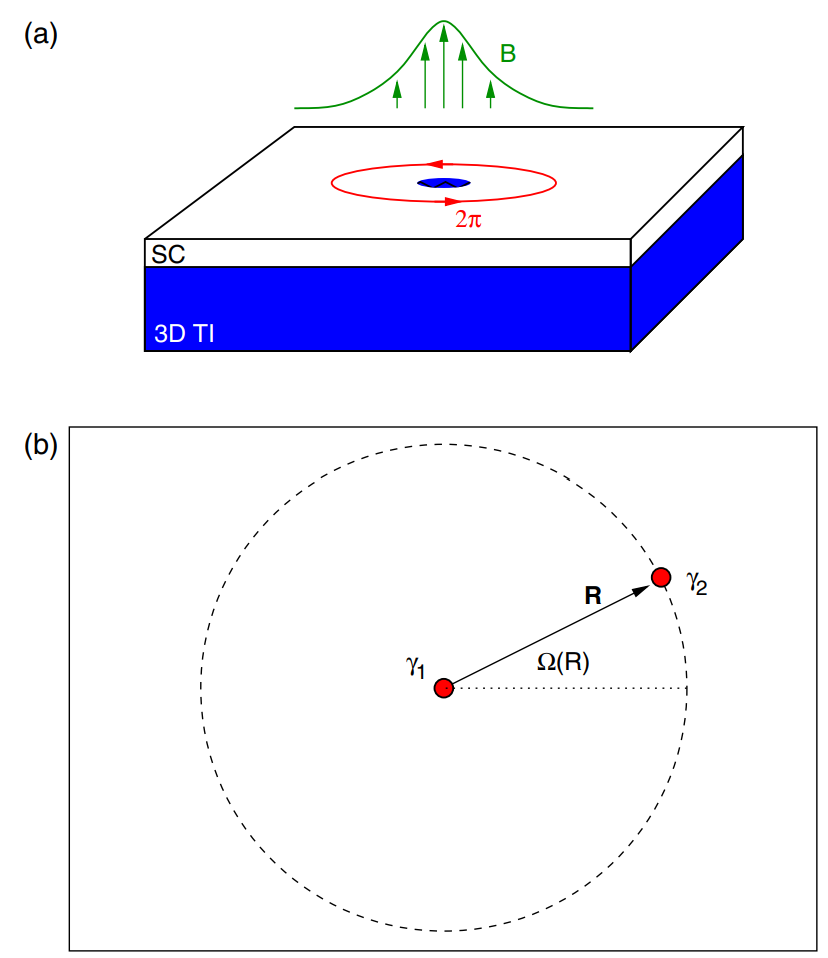
\includegraphics[scale=1]{2}
\caption{\small (a) Schemetic setup of the Fu-Kane model with an Abrikosov vortex. The bulk is a three-dimensional topological insulator and is covered by a thin layer of superconducting film. The phase winding around the core of the vortex is $2\pi$. (b) A vortex with Majorana zero mode $\gamma_2$ encircles a vortex $\gamma_1$ at the origin. The distance vector between the two vortices is $\vec{R}$ and the angular dependence of $\vec{R}$ is $\Omega(\vec{R})$. (Figure adapted from Fig.\,10 in \cite{Review})\normalsize}
\end{figure}

%\begin{align}
%\xi_{\vec{r}} = \frac{A}{\sqrt{2}}\bmat{
%\exp(-i(\alpha/2 - \pi/4))\\
%\exp(i(\alpha/2 - \pi/4))
%}\, \exp\left(
%-\int_0^r \Delta_0(r')\, dr'
%\right)\,,
%\end{align}
%which is normalizable. We can verify this step, we shall write operators in polar coordinates, 
%\begin{align}
%p_+ = -ie^{i\theta} \left( \pd_r + \frac{i}{r}\pd_\theta\right)\,,\qquad p_- = \,.
%\end{align}
%Let us consider
%\begin{align}
%\xi_{\vec{r}} = \bmat{u(r,\theta)\\v(r,\theta)}\,,
%\end{align}
%then we see that we require 
%\begin{align}
%\begin{cases}
%\Delta(\vec{r})\, u + p_- v = 0\\
%\Delta^*(\vec{r})\, v - p_+u = 0\\
%\end{cases}\,.
%\end{align}
%We solve the system by ansatz
%\begin{align}
%u(r,\theta) = e^{-i\varphi} f(r) \,,\qquad
%v(r,\theta) = e^{i\varphi} f(r)\,.
%\end{align}
%Then we see that
%\begin{align}
%s
%\end{align}

\section{Vortex Exchange and Braiding}
In this section, we will discuss the exchange statistics of the vortices, and thus the MZMs, as seen in the Ku-Kane model in section 4.1. As mentioned in the beginning of the chapter, the exchange statistics of the MZMs are used for manipulating quantum information stored in the MZMs in a topological fashion.\\

We begin by considering the effect of a vortex (represented by MZM $\gamma_2$) encircling another one (MZM $\gamma_1$) located at the origin. Schematically, this is visualized as Fig.\,4.1(b). Here we will assume the distance between the two vortices is long enough such that the splitting of the zero-mode energies due to wavefunction overlap is negligible. Given the setup, we can rewrite the angle argument in (4.8), 
\begin{align}
\alpha(\vec{R}) = \alpha_0 + \Omega(\vec{R}) + \pi\,,
\end{align}
where $\alpha_0$ is an arbitrary constant phase offset. To simplify calculation, we take $\alpha_0 = -\pi/2$ such that $\xi_{0\vec{r}}$ from (4.15) now takes the form
\begin{align}
\xi_{0\vec{r}}(\vec{R}) = \bmat{\exp(-i\Omega/2)\\
\exp(i\Omega/2)
}\, f(r)\,.
\end{align}
Assume further that the encircling process is adiabatic, parametrized by time $t \in [0,T]$ for one counterclockwise cycle, we then can define and compute the Berry phase acquired by the Majorana wavefunction, 
\begin{align}
\gamma(C) \coloneqq - \Im\left( 
\oint_C \langle \xi_{0{\vec{r}}}(\vec{R})|\nabla_{\vec{R}} \, \xi_{0\vec{r}}(\vec{R}\rangle \cdot d\vec{R}\right) - i \ln 
\left(
\langle \xi_{0\vec{r}}(\vec{R}(t=0)) \, |\,\xi_{0\vec{r}}(\vec{R}(t=T)\rangle 
\right)
\,.
\end{align}
The second term in (4.22) is crucial for the encircling. It must be included in order to account for the fact that $\xi_{0\xi}(\vec{R})$ is not single-valued as $\Omega \to \Omega +2\pi$ in one cycle. That is, WLOG, assume $\Omega(t=0) = 0$ and $\Omega(t=T) = 2\pi$,
\begin{align}
-i \ln 
\left(
\langle \xi_{0\vec{r}}(\vec{R}(t=0)) \, |\,\xi_{0\vec{r}}(\vec{R}(t=T)\rangle 
\right) =- i\ln \left(\frac{
e^{-i\pi} + e^{i\pi}}{2}
\right) = \pi\,.
\end{align}
On the other hand, it is not hard to show that the first term in (4.22) evaluate to zero, thus 
\begin{align}
\gamma(C) = \pi
\end{align}
for a single cycle. Thus, we conclude that being encircled by another singly quantized vortex at a distance $\vec{R}$ away, a given singly quantized vortex MZM wavefunction changes its sign. This statement holds true for both the MZM at the origin and the one performing the encircling motion as shown in Fig.\,4.1(b). Therefore, we can encode the spatial encircling process of these two Majorana particles as
\begin{align}
\gamma_1 \mapsto - \gamma_1\,,\qquad
\gamma_2\mapsto -\gamma_2\,.
\end{align}

\begin{figure}[b]
\centering
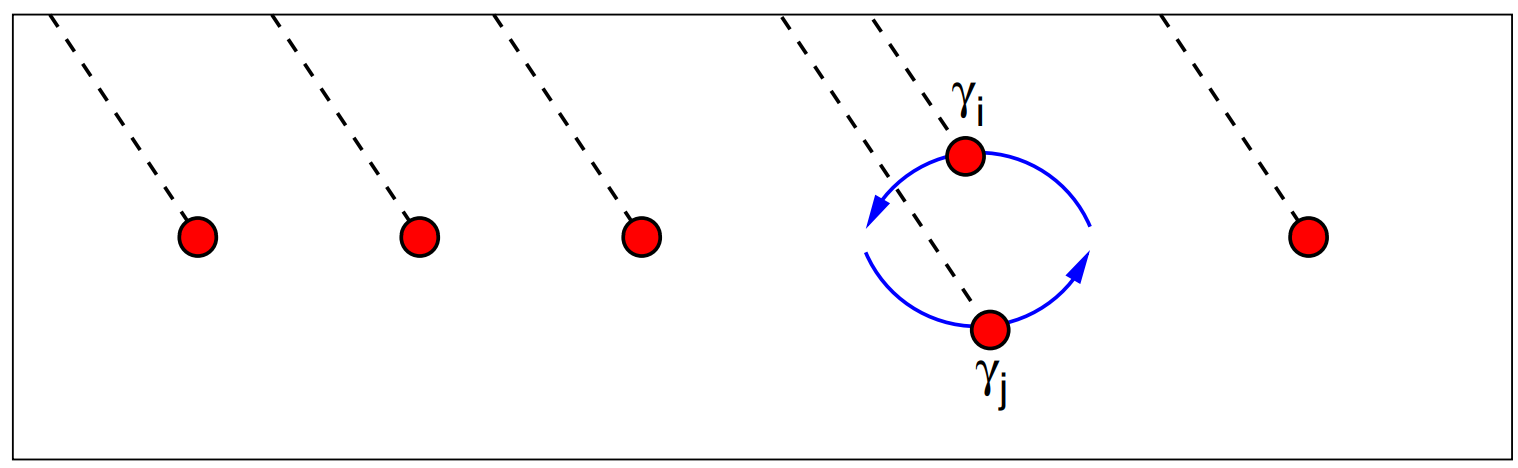
\includegraphics[scale=0.45]{3}
\caption{\small Exchanging Majorana particles $\gamma_i$ and $\gamma_j$. The red circles represent Majorana particles, and the dashed lines represent their branch cut in the wavefunction. As indicated by the blue curves, the action of exchanging necessarily cross the branch cut. (Figure adapted from Fig.\,11 in \cite{Review}.)\normalsize}
\end{figure}

In general, for a set of $2N$ many Majorana particles denoted by $\gamma_k$, we can encode the encircling operation in which $\gamma_j$ encircles $\gamma_i$ one cycle by a unitary transformation
\begin{align}
U_{ij} =\gamma_i \gamma_j\,.
\end{align}
such that 
\begin{align}
\gamma_k\mapsto U_{ij} \gamma_{k} U_{ij}^\dagger=(-1)^{\delta_{jk}+\delta_{ik}} \gamma_k \,,
\end{align}
in such a process. Referencing to Fig.\,4.2, an encircling process corresponds to a complete $2\pi$ cycle, then an spatial position exchange of $\gamma_i$ and $\gamma_j$ can be understood as half of a encircling operation, and two of such subsequent exchange processes in the same orientation (both counterclockwise or both counterclockwise) then constitutes a complete encircling process. A unitary operation that encode the exchange process is thus
\begin{align}
T_{ij} = (U_{ij})^{1/2} = \frac{1}{\sqrt{2}}\left( 1+ \gamma_i \gamma_j\right)\,.
\end{align} 
Applying $T_{ij}$ to the states $\gamma_k,\, \gamma_i,\, \gamma_j$ for $k\neq i,j$ generates the exchange statistics of the Majorana particles
\begin{align}
\gamma_i \mapsto -\gamma_j \,,\qquad
\gamma_j \mapsto \gamma_i \,,\qquad
\gamma_k \mapsto \gamma_k\,.
\end{align}
We have finally obtain the main result of this note. Eq.\,(4.29) was first derived by D.\,A.\,Ivanov in his paper \textit{Non-Abelian Statistics of Half-Quantum Vortices in p-Wave Superconductors}. It is straight forward to check that we have $T_{12}T_{23} \neq T_{23}T_{12}$, thus the braid group obtained from the exchange operators $\{T_{ij}\}$ is non-Abelian.

\section{Braiding MZMs for Quantum Information Manipulation}
As mentioned earlier in this chapter, the braid group realized by braiding MZMs is not rich enough for building a universal quantum computer. We shall illustrate this effect with a simple example in this section. \\

We consider a system that has four MZMs, labeled as $\gamma_i$ for $i\in \N_4$. The MZMs can be thought of localized in the vortices on a superconducting surface. As seen from section 3.2, we think of the MZMs as pairs forming ordinary fermions. In this case, we define the annihilation operators for the ordinary fermions,
\begin{align}
c_a = \frac{1}{2}\left(\gamma_1 + i\gamma_2\right)\,,\qquad
c_b = \frac{1}{2}\left(\gamma_3 + i\gamma_4\right)\,.
\end{align} 
Now we can consider the two-dimensional Hilbert space spanned by the eigenstates $|n_a,\, n_b\rangle$ of the number operators of the ordinary fermions, and we will discuss the operations on these states. The action of encircling $\gamma_3$ around $\gamma_1$ is implemented by 
\begin{align}
U_{31} = \gamma_3 \gamma_1 = \left( c_a^\dagger + c_a\right) \left(c_b^\dagger+ c_b\right)\,,
\end{align}
then acting $U_{31}$ on a generic state $|n_a,\, n_b\rangle$ gives
\begin{align}
U_{31}|n_a,\,n_b\rangle = (-1)^{n_a} |\bar{n}_a, \, \bar{n}_b\rangle\,,
\end{align}
where we have written
\begin{align}
\bar{n} = (1-n)\text{\,mod\,} 2\,.
\end{align}
We notice here $\gamma_3$ and $\gamma_1$ ``belong" to different ordinary fermions. The action of encircling $\gamma_3$ around $\gamma_1$ reverses the occupancy of site $a$ and $b$, and might introduce a phase. In contrast, we can encircle $\gamma_1$ around $\gamma_2$, which are the two MZMs constituting $c_a$ fermion. The encircling process is encoded by 
\begin{align}
U_{21} = \gamma_2 \gamma_1 =-i \left(c_a -c_a^\dagger \right) \left(c_a+c_a^\dagger\right)\,,
\end{align}
from which we see that 
\begin{align}
U_{21}|n_a,\, n_b\rangle = -i\left(c_a^2 + c_ac_a^\dagger - c_a^\dagger c_a + c_a^\dagger{}^2\right)\, |n_a,\, n_b\rangle \propto |n_a,\, n_b\rangle
\end{align}
merely change the phase of $|n_a,\, n_b\rangle$. The effect of exchanging the MZMs is similar, 
\begin{align}
T_{31}|n_a,\, n_b\rangle = \frac{1}{\sqrt{2}}\left( |n_a,\, n_b\rangle + (-1)^{n_a} |\bar{n}_a,\, \bar{n}_b\rangle\right)\,,\qquad
T_{21} |n_a,\, n_b\rangle \propto |n_a,\, n_b\rangle\,.
\end{align}
We see that $T_{31}$, exchanging MZMs belonging to different regular fermions, creates an entangled state; While $T_{21}$, exchanging MZMs constituting $c_a$, only changes the phase of the given state. Thus it is easy to see that $T_{21}$ and $U_{21}$ are linearly dependent as operators. From the structure seen in (4.32), (4.35), and (4.36), we thus conclude that the set of exchange and encircling operators does able to generate nontrivial manipulations, but it does not form a complete set to manipulate states $|n_a,\, n_b\rangle$ in the two-dimensional complex Hilbert space (as one shall expect four different types of manipulations, such as that given by the set of Pauli matrices with the identity matrix). Therefore, we conclude that the braid group obtained by exchange statistics of the MZMs is not rich enough to build a universal quantum computer. However, we note that there exists theoretical approach, using the braid group obtained from the non-Abelian exchange statistics of Fibonacci anyons, to construct a universal quantum computer. Similar to the Majorana fermions, Fibonacci anyons can also be regarded as solid-state realizations of emergent particles \cite{Nayak}. 

\section*{Summary}
In this note, we started from the particle physics point of view to study properties of Majorana fermions, where we found that they are chargeless and are viewed as their own antiparticles. That motivated the study of Majorana fermions in solid-state physics, where we saw that the particle-antiparticle structure of Majorana fermions can be obtained by decomposing a regular fermion into is real and imaginary parts. We then explored these features of Majorana fermions under the BdG formalism for superconductors. In particular, we found that Majorana fermions were naturally used as quasiparticles to describe excitations in the BdG theory.\\

Since then, we focused on the Majorana zero modes, which were found as eigenstates of the BdG Hamiltonian. Kitaev chain model helped us to understand that the MZMs naturally occur in pairs. Then we used the Fu-Kane model with Abrikosov vortices to study the exchange statistics of the MZMs, and ended with discussing the limitation of using the braid group obtained from exchanging MZMs to manipulate quantum information.\\

Undoubtedly, the search for experimental realization of the Majorana fermions, the MZMs, and the exchange statistics of the MZMs are ongoing research topics in physics. The discovery of particles or quasiparticles governed by Majorana's formalism would carry profound scientific implications and has attracted considerable interest in recent years. For more related topics and discussion of Majorana fermions in experimental contexts, we refer interested readers to \cite{Review, FuKane, HasanKane, Sankar, Motome}.

\begin{thebibliography}{9}
\bibitem{Review} Elliott, S.\,R., and M.\,Franz, Rev.\,Mod.\,Phys.\,\textbf{87}, 137 (2015).
\bibitem{KitaevChain} Kitaev, A., Phys.\,Usp.\,\textbf{44}, 131 (2001).
\bibitem{FuKane} Fu, L., and C.\,L.\,Kane, Phys.\,Rev.\,Lett.\,\textbf{100}, 096407 (2008).
\bibitem{HasanKane} Hasan, M.\,Z., and C.\,L.\,Kane, Rev.\,Mod.\,Phys.\,\textbf{82}, 3045 (2010).
\bibitem{Nayak}Nayak, C., S.\,H.\,Simon, A.\,Stern, M.\,Freedman, and S.\,Das Sarma, Rev. Mod. Phys. \textbf{80}, 1083 (2008).
\bibitem{Sankar}Sarma, S., M.\,Freedman, and C.\,Nayak, npj Quantum Inf.\,\textbf{1}, 15001 (2015).
\bibitem{Motome}Motome, Y., and J.\,Nasu, J.\,Phys.\,Soc.\,Jpn.\,\textbf{89}, 012002 (2020).
\end{thebibliography}
\end{document}


